\section{Multipole Truncation Analysis}
While the extraction of the structure functions is model independent, 
assumptions on the partial waves of the background and other resonances have to be made
in order to extract quantities such as the coefficients of the legendre expansion of the 
structure functions or the electromagnetic multipoles.
 

\subsection{Legendre expansion}
\label{sec:legendre}
In order to extract the multipoles, the structure functions were fitted
with orthogonal Legendre polynomials with $\ell$ up to d-waves (both the cases
$\ell\le 1$ and $\ell \le 2$ have been considered).
In the case of $\ell \le 1$ the expansion is:
$$
\begin{array}{l c l}
\sigma_T + \epsilon\sigma_L & = & A_0 + A_1P_1(cos\theta) + A_2P_2(cos\theta) \\
\sigma_{TT}                 & = & C_0 \\
\sigma_{LT}                 & = & D_0 + D_1P_1(cos\theta)  \\
\end{array}
$$

In the case of $\ell \le 2$ the expansion is:
$$
\begin{array}{l c l}
\sigma_T + \epsilon\sigma_L & = & A_0 + A_1P_1(cos\theta) + A_2P_2(cos\theta) + A_2P_3(cos\theta) + A_3P_4(cos\theta)\\
\sigma_{TT}                 & = & C_0 + C_1P_1(cos\theta) \\
\sigma_{LT}                 & = & D_0 + D_1P_1(cos\theta) + D_2P_2(cos\theta) \\
\end{array}
$$


Figures \ref{fig:Sigma_lpt_Q2_2.40},  \ref{fig:Sigma_tt_Q2_2.40} and \ref{fig:Sigma_lt_Q2_2.40} show 
the fits for $\sigma_L + \epsilon\sigma_T$, $\sigma_{TT}$ and $\sigma_{LT}$ for different 
$W$ at $Q^2 = 2.4$ GeV$^2$. 
\F{fig:chi2_rtm} shows the obtained and the expected $\chi^2/\nu$ distributions for the various response functions.

To see the fits for $\sigma_L + \epsilon\sigma_T$, $\sigma_{TT}$ and $\sigma_{LT}$ for all the 
$Q^2$ bins and $\ell\le 1$ and $\ell \le 2$ cases, see
\begin{verbatim} 
http://www.jlab.org/~ungaro/pi0eprod/responses
\end{verbatim}

\begin{figure}[h]
 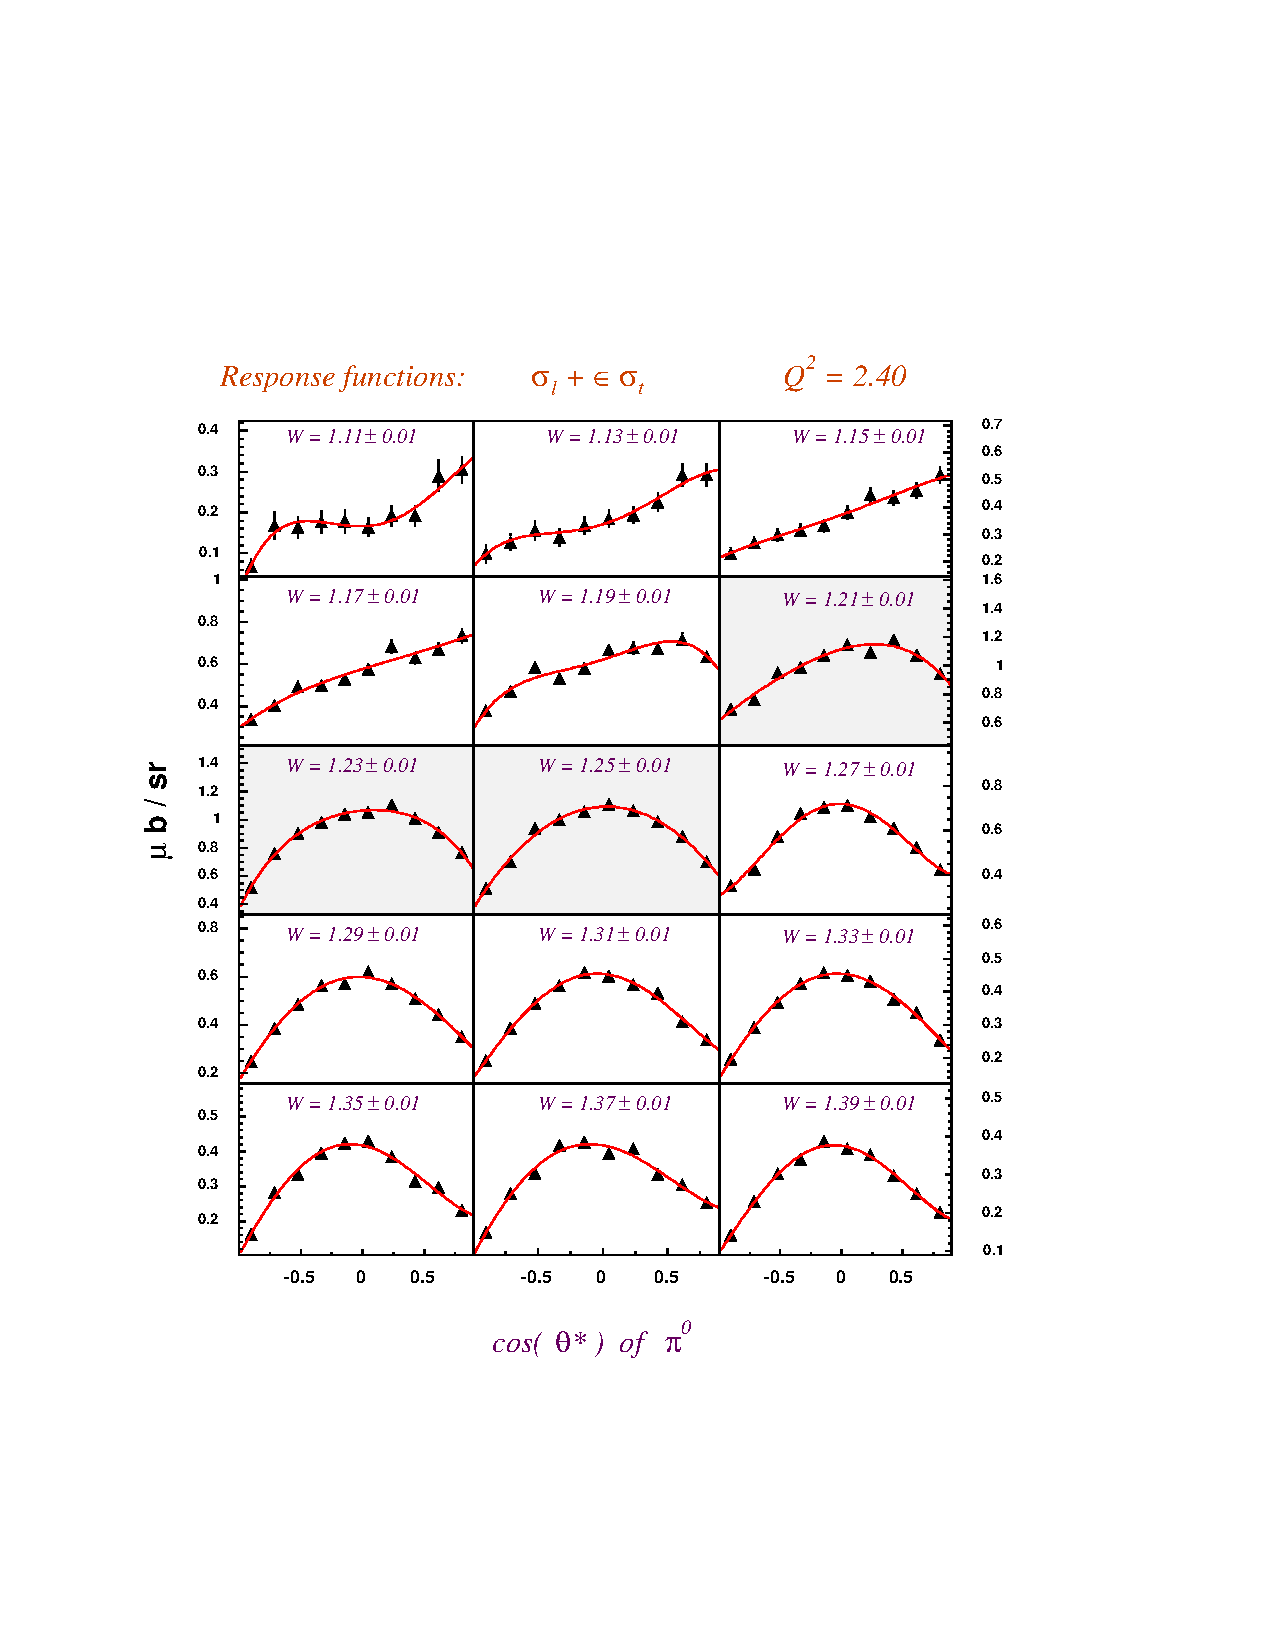
\includegraphics[width = 15cm, bb=0 100 500 640]{analysis/img/Sigma_lpt_Q2_2.40}
  \caption[$\sigma_L + \epsilon\sigma_T$ for different $W$ at $Q^2 = 2.4$ GeV$^2$]
          { $\sigma_L + \epsilon\sigma_T$ for different $W$ at $Q^2 = 2.4$ GeV$^2$. 
		     The legendre expansion (red line fit) is: 
		     $\sigma_T + \epsilon\sigma_L = A_0 + A_1P_1(cos\theta) + A_2P_2(cos\theta) 
		                                        + A_2P_3(cos\theta) + A_3P_4(cos\theta)$.\\
                     Regions near the $\Delta $ region are shaded.}
 \label{fig:Sigma_lpt_Q2_2.40}
\end{figure}



\begin{figure}[h]
 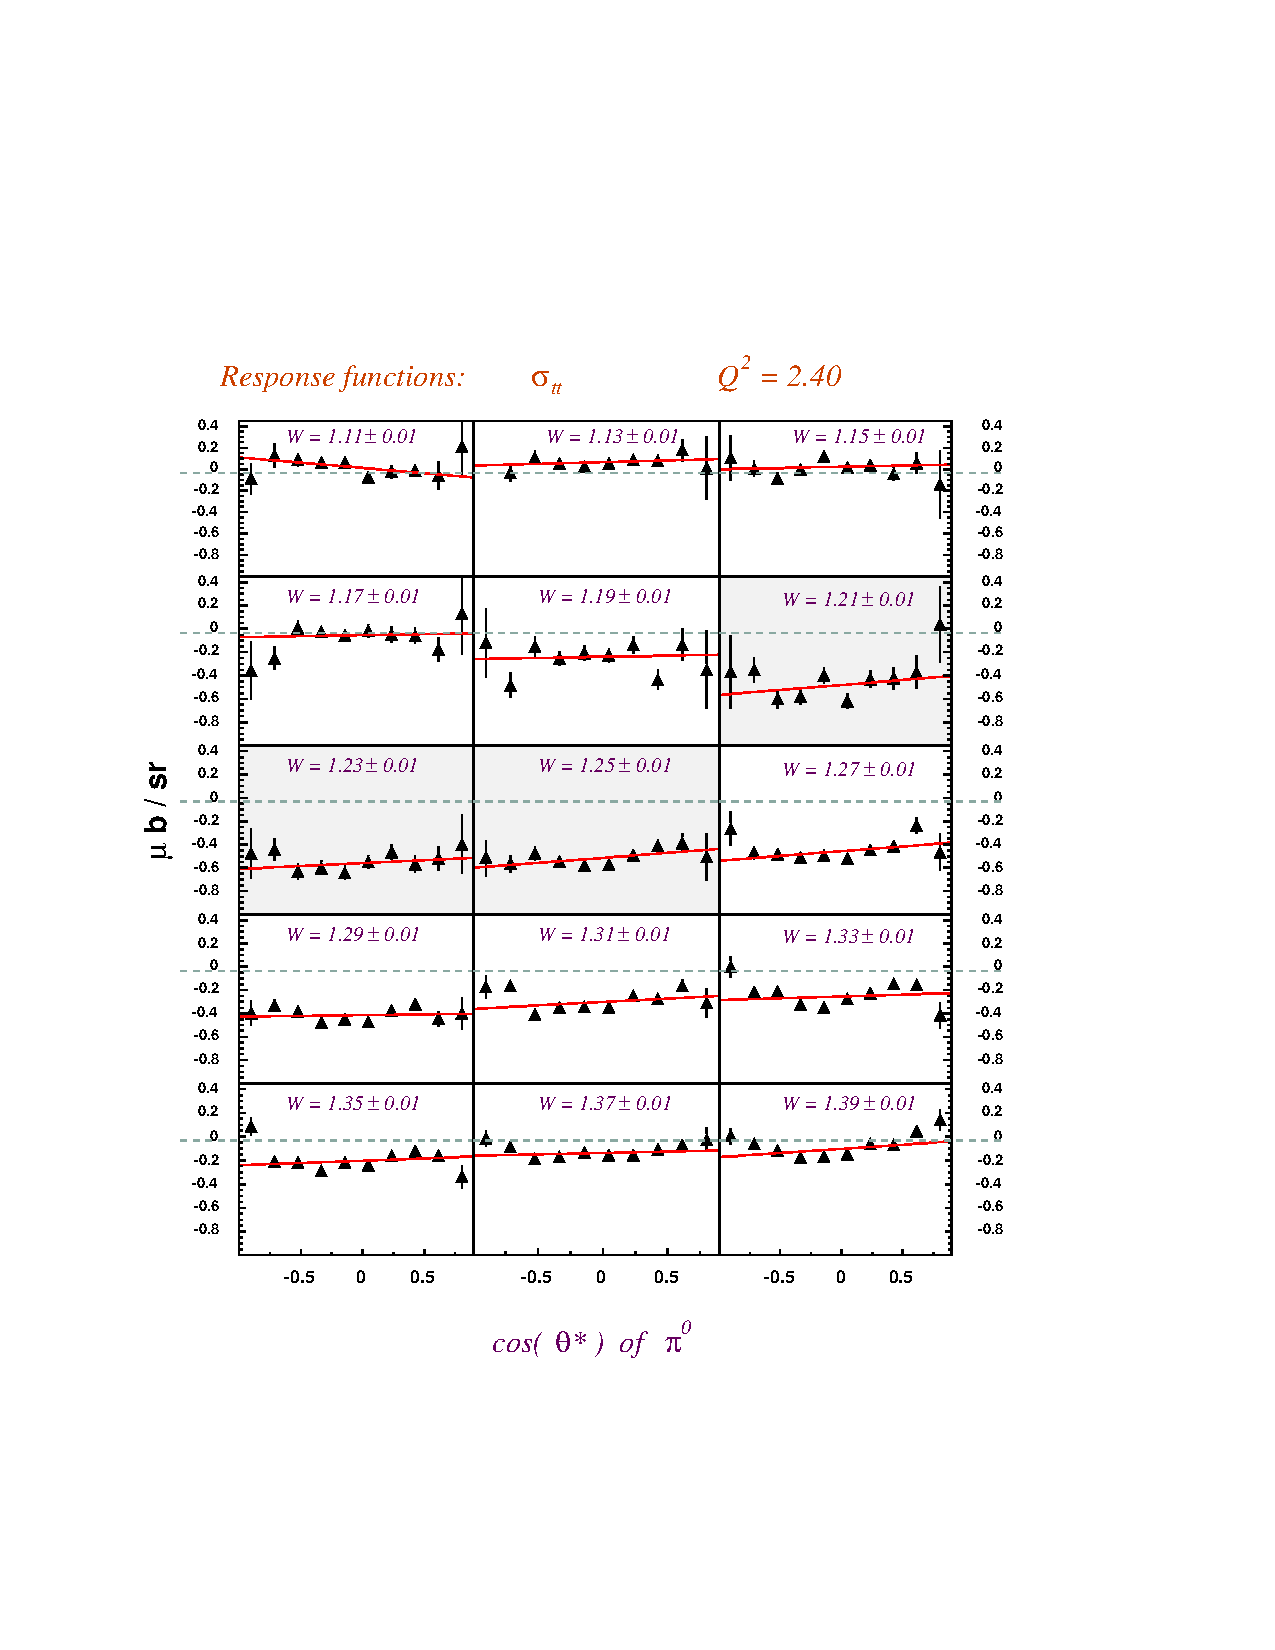
\includegraphics[width = 15cm, bb=0 100 500 640]{analysis/img/Sigma_tt_Q2_2.40}
  \caption[$\sigma_{TT}$ for different $W$ at $Q^2 = 2.4$ GeV$^2$]
          { $\sigma_{TT}$ for different $W$ at $Q^2 = 2.4$ GeV$^2$. 
		     The legendre expansion (red line fit) is: 
		     $\sigma_{TT} = C_0 + C_1P_1(cos\theta)$.	  \\
	             Regions near the $\Delta $ region are shaded.}
 \label{fig:Sigma_tt_Q2_2.40}
\end{figure}


\begin{figure}[h]
 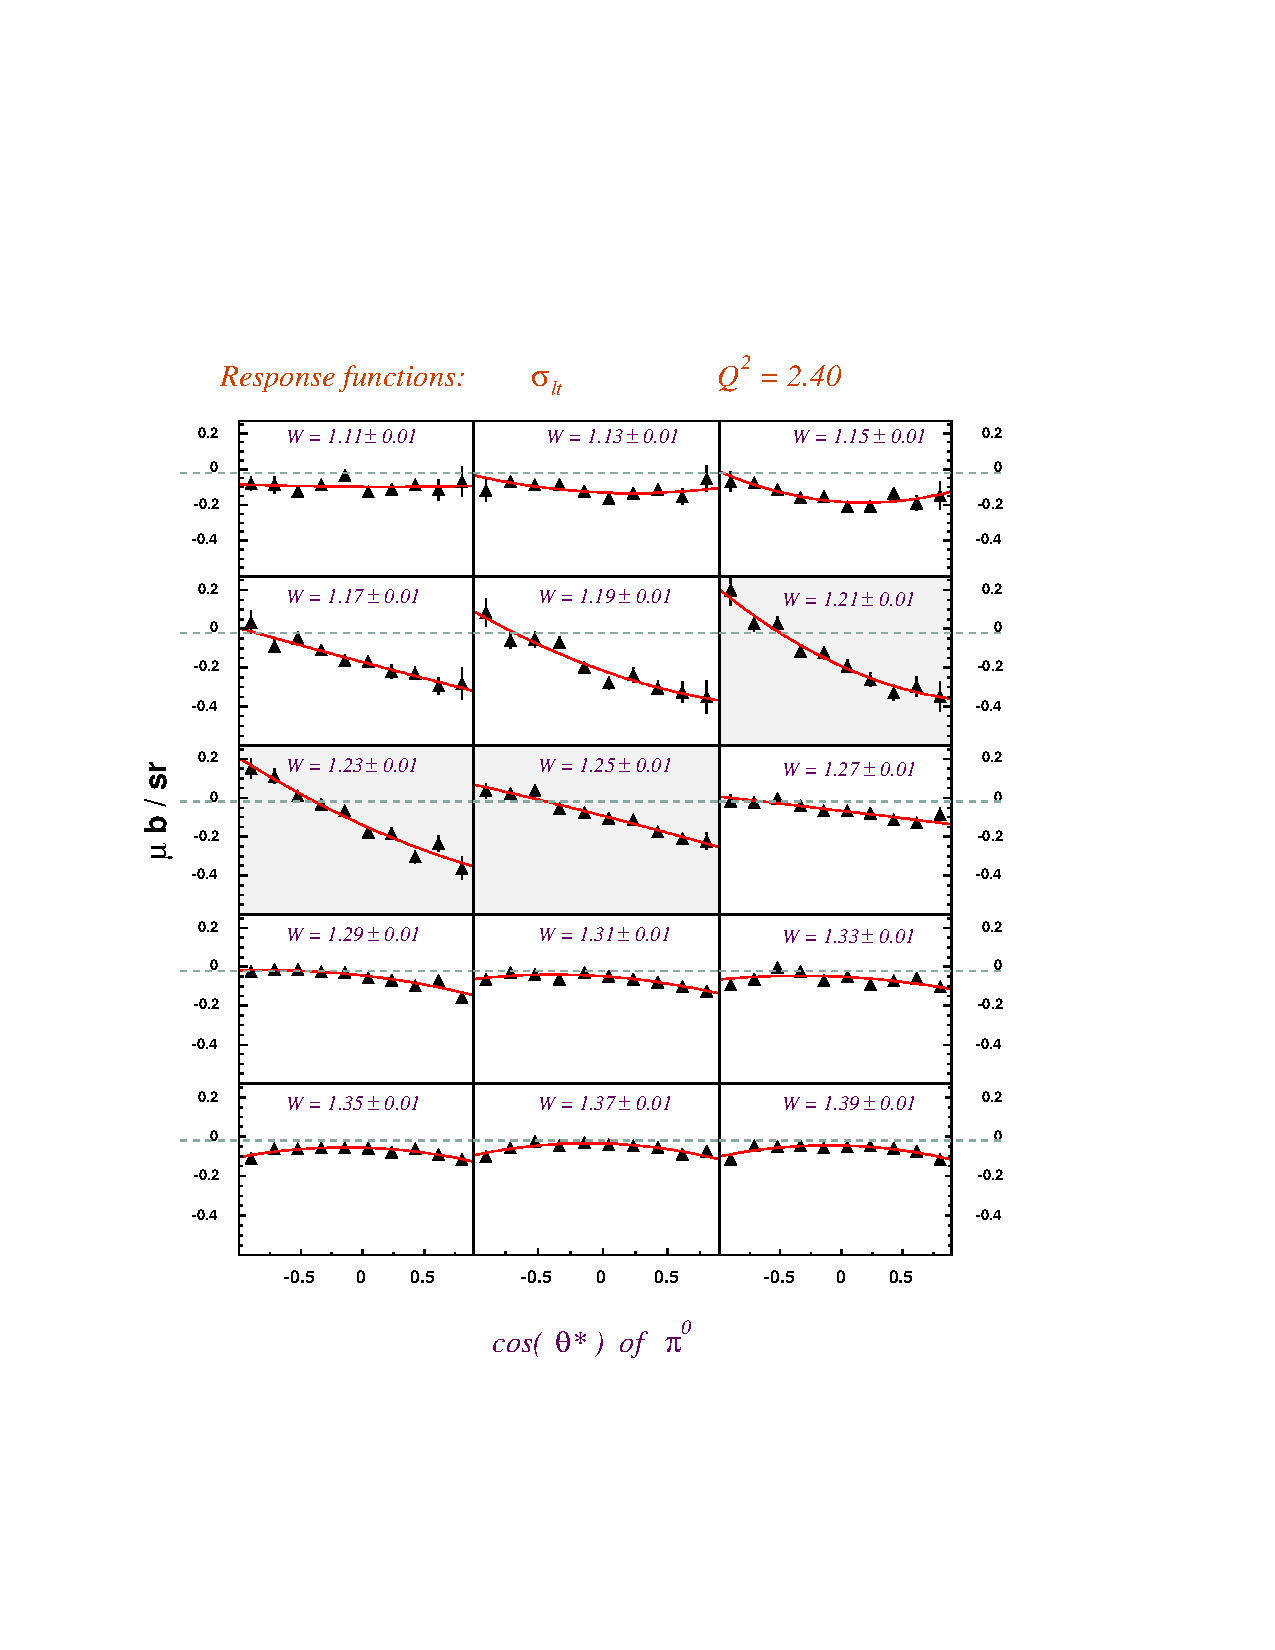
\includegraphics[width = 15cm, bb=0 100 500 640]{analysis/img/Sigma_lt_Q2_2.40}
  \caption[$\sigma_{LT}$ for different $W$ at $Q^2 = 2.4$ GeV$^2$]
          { $\sigma_{LT}$ for different $W$ at $Q^2 = 2.4$ GeV$^2$. 
		     The legendre expansion (red line fit) is: 
		     $\sigma_{LT} = D_0 + D_1P_1(cos\theta) + D_2P_2(cos\theta) $.\\
	             Regions near the $\Delta $ region are shaded.}
 \label{fig:Sigma_lt_Q2_2.40}
\end{figure}

\begin{figure}[h]
 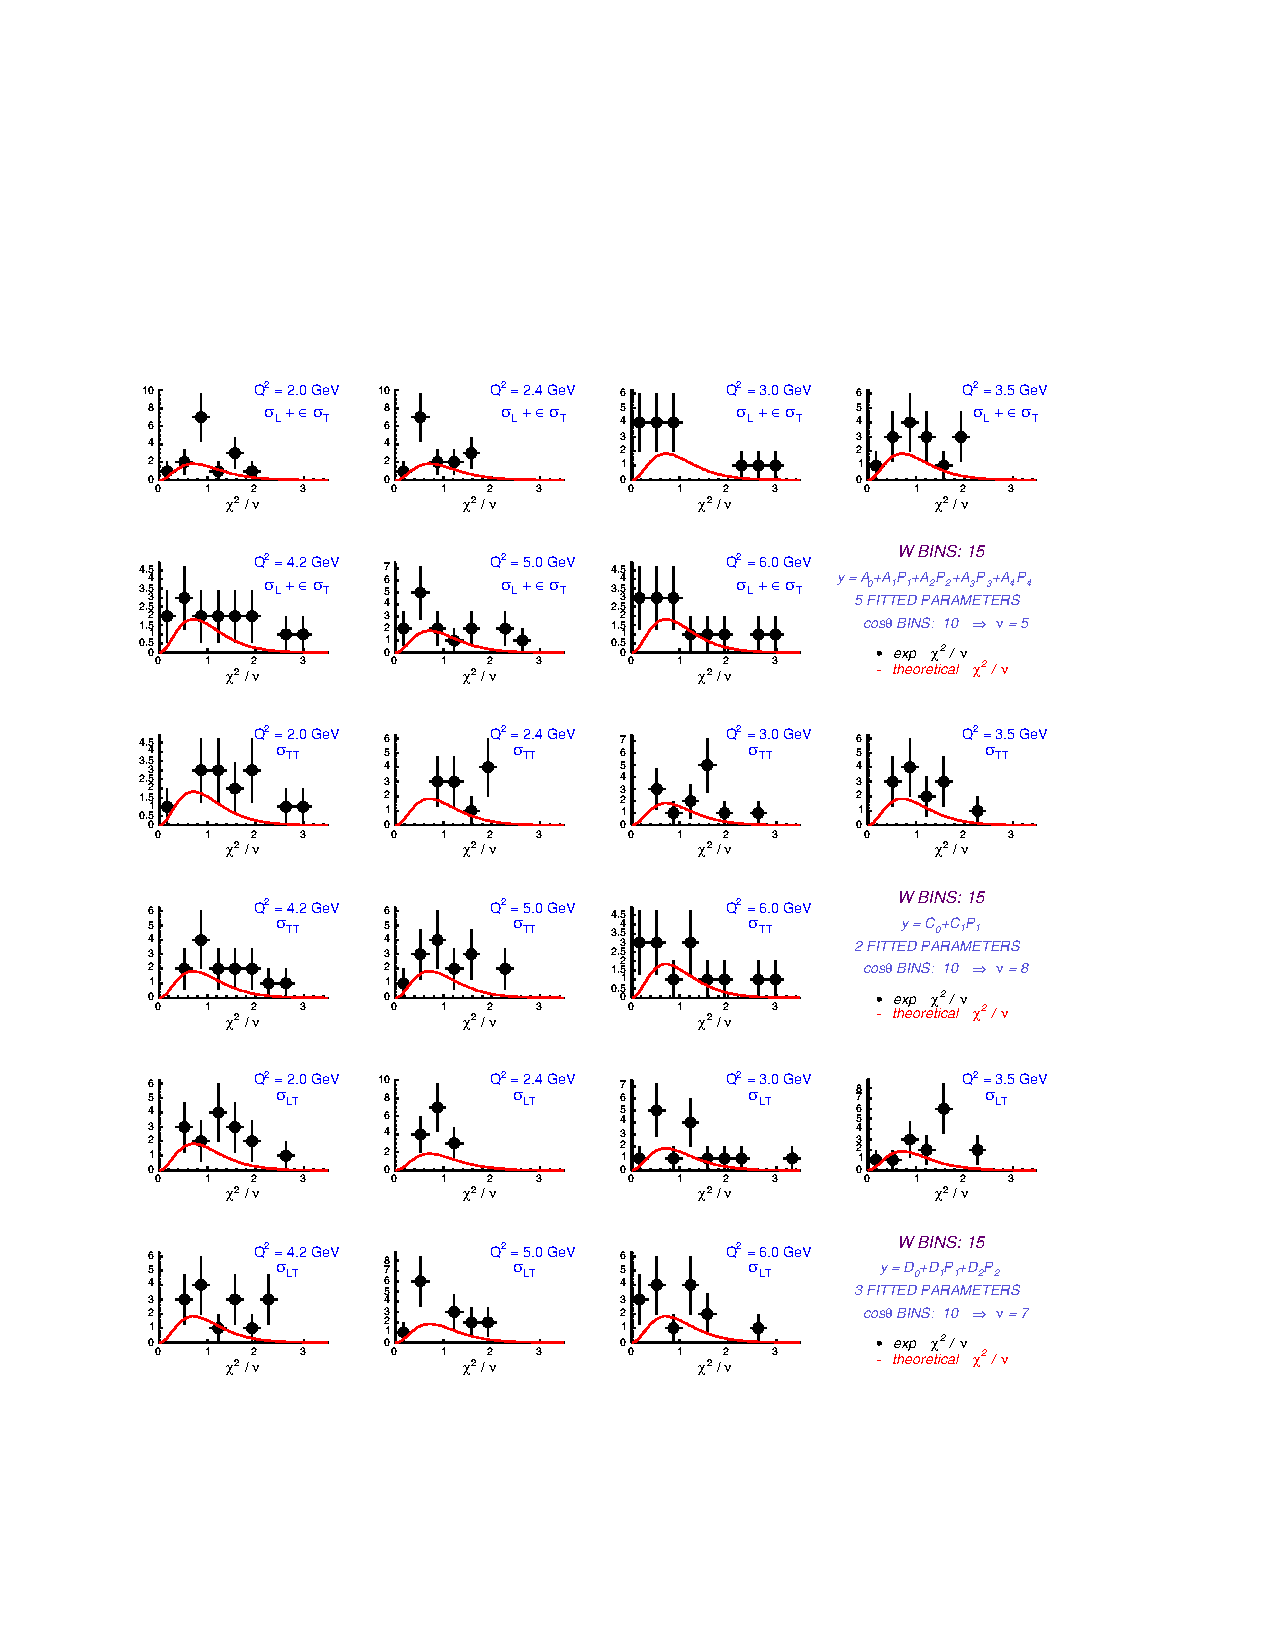
\includegraphics[width = 15.4cm, bb=40 100 530 640]{analysis/img/chi2_rtm} 
  \caption[Reduced $\chi^2$ distribution of the Legendre fits]
          { Reduced $\chi^2$ distribution of the Legendre fits. 
	             The $\sigma_L + \epsilon\sigma_T$, $\sigma_{TT}$ and  $\sigma_{LT}$ have respectively
		     5, 8, and 7 degrees of freedom. Each plot has only 15 points (there are 15 $W$ bins)
		     so the statistic of the $\chi^2/\nu $ distributions is poor. The red line is the expected 
		     $\chi^2$ distribution.}
 \label{fig:chi2_rtm}
\end{figure}

\cia
\F{fig:Coefficients_q2.4} shows the coefficients of the Legendre expansion for $Q^2=2.4$ GeV$^2$.
The coefficient $A_0 $, proportional to $M_{1+}$ if $\sigma_L << \sigma_T$ (see Eqn \ref{eqno:m1dominance}) and to the total c.m. cross section, 
shows the characteristic
resonance behaviour at the peak of the $\Delta$.


\begin{figure}[h]
 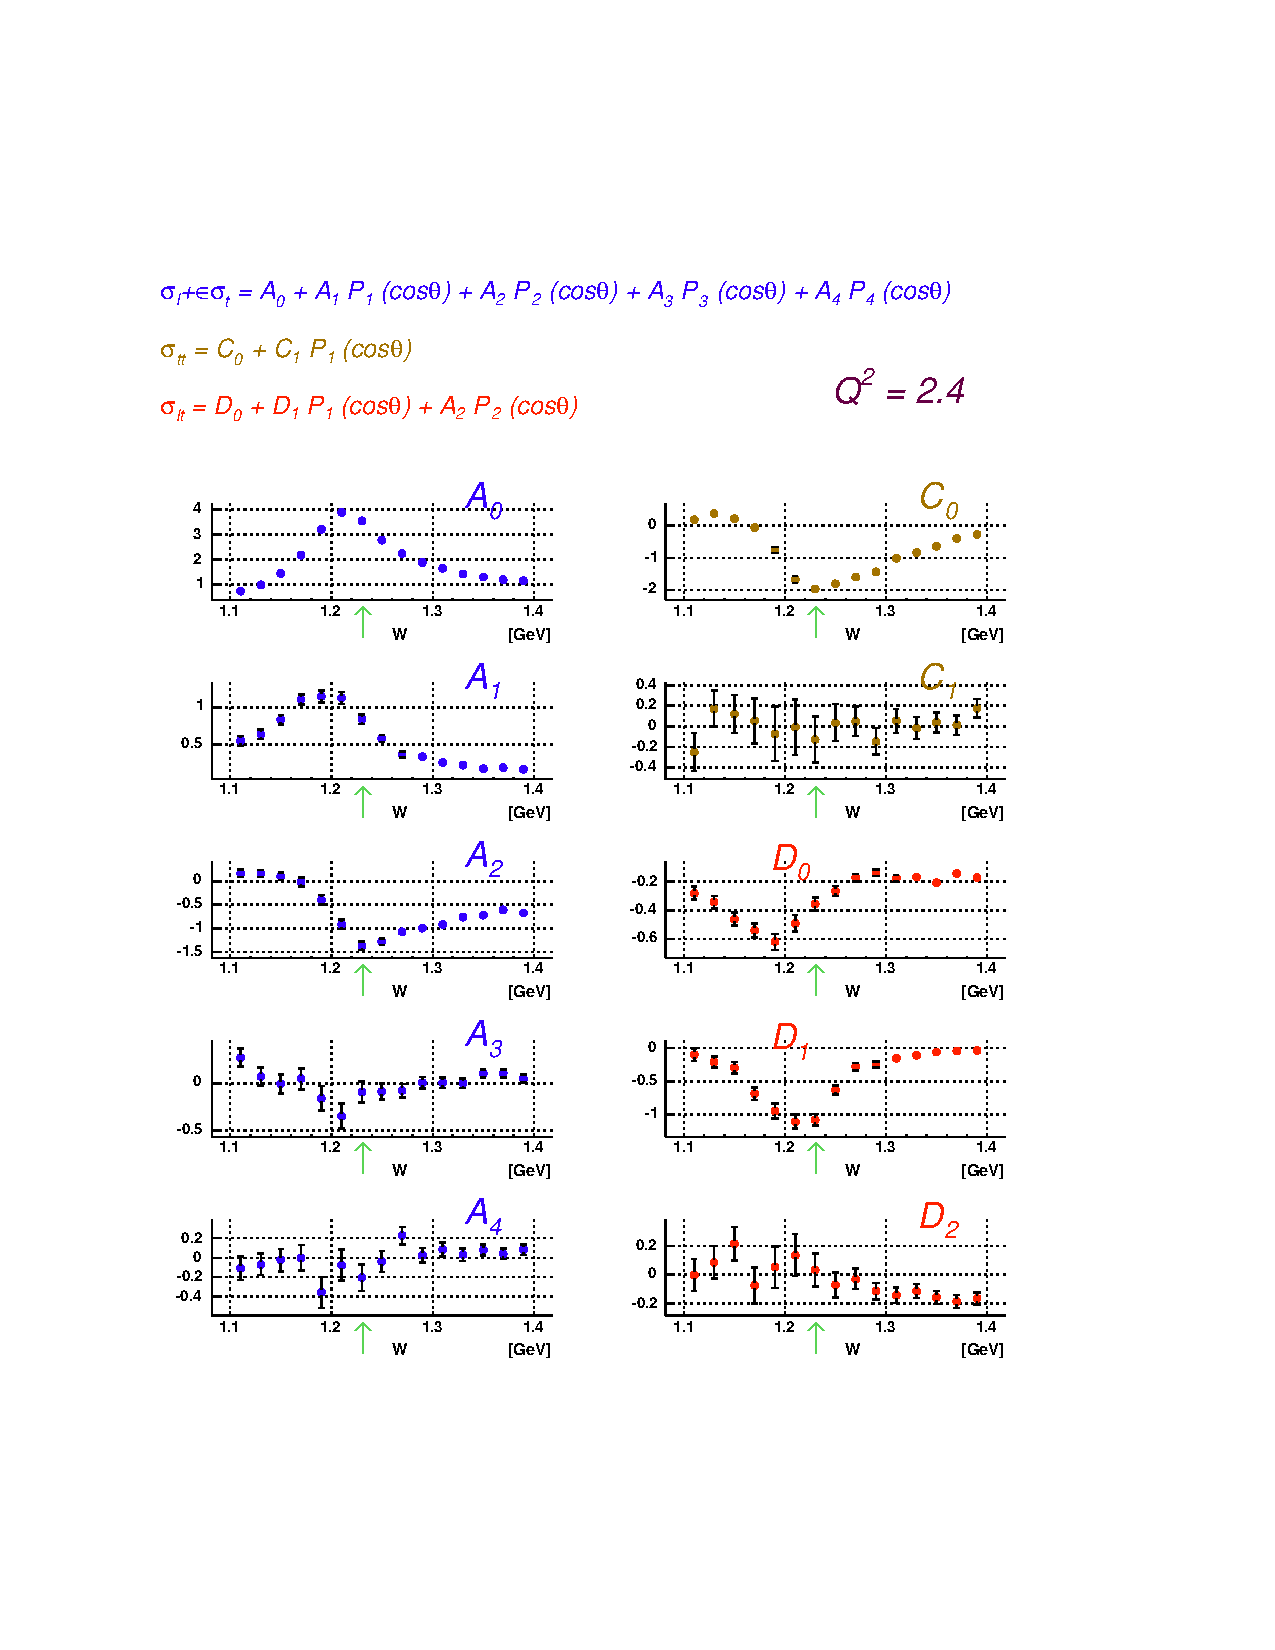
\includegraphics[width = 15cm, bb=0 100 540 700]{analysis/img/Coefficients_q2.4}
  \caption[Legendre coefficients at $Q^2 = 2.4$ GeV$^2$]
          { Legendre coefficients at $Q^2 = 2.4$ GeV$^2$. The green arrow shows the $\Delta$ mass
	             position. The coefficient $A_0$ is proportional to $M_{1+}$ and to the total c.m. cross section.}
 \label{fig:Coefficients_q2.4}
\end{figure}  


\cia
See    \begin{verbatim} 
http://www.jlab.org/~ungaro/pi0eprod/coefficients
\end{verbatim}
for the plots of the various coefficients for different cuts used in the analysis.
















